

\documentclass[11pt]{article}

\title{ Advancing predictive physical modeling through focused development of model systems to drive new modeling innovations}

\usepackage[top=0.5in, bottom=0.5in, left=0.5in, right=0.5in]{geometry}
\usepackage{helvet}
\usepackage{url} % hypderref?
\usepackage{graphicx}
\graphicspath{{figures/}} % The figures are in a figures/ subdirectory.
\renewcommand{\familydefault}{\sfdefault}
\pagestyle{empty}
%\pagestyle{plain}

% Fancy page-width tables
\usepackage{tabularx}

% Use a package for framed boxes
\usepackage{mdframed}

\usepackage[T1]{fontenc}
\usepackage{amssymb}


\usepackage{setspace}
\usepackage{microtype}

\usepackage{amsfonts}
\usepackage{amsmath}

\usepackage{floatrow}

\usepackage[normalem]{ulem} % for nci.bst

\usepackage{sidecap}
\usepackage[abs]{overpic}
\usepackage{wrapfig}


\usepackage{hyperref}
\hypersetup{colorlinks=true, urlcolor=black, citecolor=black, linkcolor=black}

\usepackage[numbers,sort&compress]{natbib} %comment on first run?

% \usepackage{multibib}
% %\newcites{full,sampl}{A,B}
% \newcites{sampl}{Full List of SAMPL References}
% %\newbibliography{full}

%\usepackage[round,authoryear]{natbib}
%\usepackage{cite}
%\setlength{\bibsep}{0.00in}


\newcommand{\doi}[1]{\href{http://dx.doi.org/#1}{doi:#1}}

\newcommand{\ac}[1]{{\sc \lowercase{#1}}}

\renewcommand{\baselinestretch}{.93}
%\renewcommand{\baselinestretch}{.90}
\usepackage{wrapfig}

% \usepackage{bibspacing}
% \setlength{\bibspacing}{\baselineskip}




\graphicspath{{figs/}}

\makeatletter

\newcommand{\captionfonts}{\footnotesize}

\makeatletter  % Allow the use of @ in command names
\long\def\@makecaption#1#2{%
  \vskip\abovecaptionskip
  \sbox\@tempboxa{{\captionfonts #1: #2}}%
  \ifdim \wd\@tempboxa >\hsize
    {\captionfonts #1. #2\par}
  \else
    \hbox to\hsize{\hfil\box\@tempboxa\hfil}%
  \fi
  \vskip\belowcaptionskip}
\makeatother

\renewcommand{\figurename}{{\bf Figure}}

% Page numbering.
%\pagestyle{plain}
%\pagenumbering{arabic}

\setlength{\abovecaptionskip}{-5pt}

\makeatother

\renewcommand{\refname}{Bibliography and References Cited}

\setlength{\parindent}{0pt} % Don't indent first line
%\setlength{\parskip}{1ex plus 0.5ex minus 0.2ex} % Add some space between paragraphs
\setlength{\parskip}{0.8ex} % Add some space between paragraphs

%%%%%%%%%%%%%%%%%%%%% c-bun's additions
\newcommand{\comment}[1]{\textit{\textcolor{red}{#1}}}
%%%%%%%%%%%%%%%%%%%%% end c-bun's additions

\begin{document}

%%%%%%%%%%%%%%%%%%%%%%%%%%%%%%%%%%%%%%%%%%%%%%%%%%%%%%%%%%%%%%%%%%%%%%%%%%%
% SPECIFIC AIMS
%%%%%%%%%%%%%%%%%%%%%%%%%%%%%%%%%%%%%%%%%%%%%%%%%%%%%%%%%%%%%%%%%%%%%%%%%%%

%{\large \bf SPECIFIC AIMS}

%\eject

%%%%%%%%%%%%%%%%%%%%%%%%%%%%%%%%%%%%%%%%%%%%%%%%%%%%%%%%%%%%%%%%%%%%%%%%%%%
% SIGNIFICANCE
%%%%%%%%%%%%%%%%%%%%%%%%%%%%%%%%%%%%%%%%%%%%%%%%%%%%%%%%%%%%%%%%%%%%%%%%%%%

% !TEX root = ./Research_and_SA.tex

% FROM THE NIH SITE:
% Is the proposed research project of high scientific quality, and is it well integrated with the proposed research training plan?
% Based on the sponsor’s description of his/her active research program, is the applicant’s proposed research project sufficiently distinct from the sponsor’s funded research for the applicant’s career stage?
% Is the research project consistent with the applicant’s stage of research development?
% Is the proposed time frame feasible to accomplish the proposed training?

\noindent \begin{center}
{\bf SPECIFIC AIMS}
\end{center}

Genetically-encoded probes have revolutionized our understanding of cellular processes. Fluorescent proteins are a powerful technology that enable tracking of protein concentration and localization over large timescales and with single-molecule resolution. Via simple genetic manipulation, virtually any protein of interest can be labeled and tracked in the cell. However, analogous techniques for study of other biomolecules through genetic encoding (e.g. RNA)  are underdeveloped. There is currently no approach suitable for tracking the diverse types of RNAs found in mammalian cells. % Amy: suggested edit: "are far less developed and there is currently no approach suitable for tracking the diverse types of RNAs found in mammalian cells."

The importance of RNA in controlling a wide range of cellular functions has only recently been realized \cite{CechNoncodingRNARevolution2014}. Signaling by messenger and noncoding RNAs in the cell is highly dependent on the location of the transcripts. It is understood that cellular machinery modulates the location of these molecules, but these processes remain difficult to elucidate \cite{Muller-McNicollHowcellsget2013a}.
%Only (SOME FRACTION HERE) of RNA are actually involved in protein synthesis, while the rest is not well understood.
This lack of understanding is due in part to the lack of tools available to image this biomolecule. Localization of RNA on a single-molecule level, and multicomponent imaging of RNA transcripts remains difficult. Existing tools utilize aptamers that are unstable in mammalian cells \cite{EtzelSyntheticRiboswitchesPlug2017}, or constructs that are too large for imaging most transcripts. Multicomponent RNA imaging is also difficult due to the design of current tools.

To address this need, \textit{I aim to develop a platform for RNA imaging that will enable facile tracking of multiple transcripts at high resolution}. Riboglow is an RNA imaging platform recently developed in the Palmer lab. It utilizes a fluorescence-quenched pair formed by cobalamin (vitamin B\textsubscript{12}) and a pendant fluorophore. In solution, this construct shows low fluorescence. When bound to the cobalamin riboswitch aptamer domain \cite{JohnsonJrB12cofactorsdirectly2012}, there is an increase in fluorescence. This tool shows promise for RNA imaging because it solves many of the problems faced by traditional RNA probes.
The platform is similar to Spinach \cite{PaigeRNAMimicsGreen2011}, Broccoli \cite{FilonovBroccoliRapidSelection2014}, and Mango \cite{AutourFluorogenicRNAMango2018,DolgosheinaRNAMangoAptamerFluorophore2014} in that it utilizes a small molecule-binding aptamer for localization, but improves on these tools because it utilizes a natural aptamer that is more stable in the cellular environment (because of its native fold).
The current gold-standard for imaging is the MS2-FP system \cite{FuscoSinglemRNAMolecules2003}, which utilizes an stem-loop-binding bacteriophage coat protein fused to a fluorescent protein. Though this technique benefits from the modularity of fluorescent proteins, it requires large constructs to concentrate the fluorescent signal (24 stem-loops are often placed in series), thus precluding its use with most RNAs.

Riboglow is already a useful tool for RNA imaging, but several drawbacks are keeping it from widespread utility. The proposed work addresses these drawbacks, and seeks to utilize improved Riboglow tools to study outstanding questions in the field of noncoding RNA. The \underline{\textit{objective}} of the work is to image noncoding RNAs as they function within living cells. My \underline{\textit{central hypothesis}} is that the Riboglow platform can be improved through chemical modification and RNA selection to provide brighter, multicomponent probes.

{\bf \underline{Aim 1.} Synthesize improved Riboglow probes.}\\
Previously developed Riboglow constructs suffered from poor signal induction and low brightness. I aim to derivatize the native cobalamin structure to produce new probe scaffolds. The linker and fluorophore will also be varied with the goal to maximize fluorescence turn-on. These new molecules will be evaluated for quenching efficiency and will be tested with native cobalamin aptamers.

{\bf \underline{Aim 2.} Adapt Riboglow for single-molecule imaging.}\\
The molecules developed in \textit{Aim 1} will be screened against libraries of aptamers to further improve probe properties. Screening will be carried out in mammalian cells via flow cytometry. Candidate probes will be verified through imaging of mRNA transcripts in living cells.

{\bf \underline{Aim 3.} Develop mutually orthogonal Riboglow probes for multicomponent imaging.}\\
In tandem with brightness optimization, I will develop mutually orthogonal probes to enable labeling of different RNA transcripts in the same cell. The power of SELEX to find selective and tight binders will be used to screen for mutually exclusive aptamer-cobalamin pairs. These pairs will be conjugated to spectrally-resolved fluorophores to enable tracking of multiple RNA simultaneously. These orthogonal probes will be used to image long noncoding RNA and mRNA as they interact in the cell.

%%% Local Variables: ***
%%% mode: latex ***
%%% TeX-master: "Research_and_SA.tex" ***
%%% End: ***

% !TEX root = ./Research_and_SA.tex

\textbf{SIGNIFICANCE}
RNA lies at the center of cellular function. Its most appreciated function is to carry protein blueprints to the ribosome for manufacture. Only recently have researchers begun to appreciate its myriad of other functions, many of which also lie at the center of important cellular processes.\cite{CechNoncodingRNARevolution2014} \comment{X, Y, and Z (maybe the proposed test systems??)} have been recently found to have crucial RNA components.
\comment{Need more on these systems here. Talk about how localization is important.}
This importance for cellular function necessitates a toolset of probes to study these RNAs as they traverse the cell.
% TODO more here. look at RNA imaging paper intros for examples.

%%%%%%%%%%%%%%%%%%%%%%%%%%%%%%%%%%%%%%%%%%%%%%%%%%%%%%%%%%%%%%%%%%%%%%%%%%%%%%%%
%Riboglow
\begin{wrapfigure}[30]{r}{9cm}
%\vspace{-0.2in}
\begin{centering}
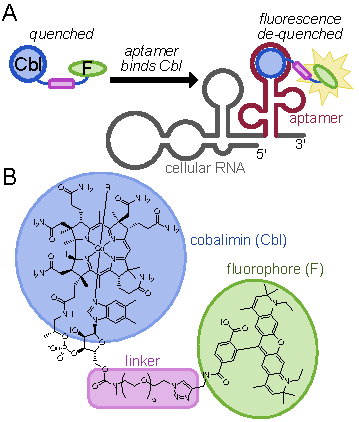
\includegraphics[width=\textwidth]{figures/fig1v2.pdf}

\end{centering}
\footnotesize
\caption{\label{figure:riboglow}
A) Cobalamin acts as a quenching and localization moiety to guide a fluorescent probe to an RNA transcript of interest. When unbound, fluorescence is quenched. In the presence of RNA tagged with the cobalamin aptamer, fluorescence is restored. B) Structure of the generation 1 Riboglow probe. A polyethylene glycol linker of five units (5xPEG) connected to the 5' hydroxly of the cobalamin ribose was used to tether an ATTO 590 fluorophore to the construct.
}
\end{wrapfigure}
%%%%%%%%%%%%%%%%%%%%%%%%%%%%%%%%%%%%%%%%%%%%%%%%%%%%%%%%%%%%%%%%%%%%%%%%%%%%%%%%

\textbf{BACKGROUND}
Protein studies benefit from a large imaging toolkit that has been developed over the last \comment{XX} years. Genetically encodable fluorescent proteins are now ubiquitous for the study of the localization of any translated target in the cell. While fluorescent proteins are a mature, well-understood technology, tools for imaging the localization of individual RNA transcripts remain limited. The most popular systems to date include dye-binding aptamers (Spinach\cite{PaigeRNAMimicsGreen2011}, Broccoli\cite{FilonovBroccoliRapidSelection2014}, and Mango\cite{AutourFluorogenicRNAMango2018,DolgosheinaRNAMangoAptamerFluorophore2014}), and RNA-binding protein fusions (MS2-FPs).\cite{FuscoSinglemRNAMolecules2003}

The most analogous to fluoresecent proteins, dye-binding aptamers utilize exogenously administered dyes that give fluorescence induction upon binding their RNA partner.\cite{PaigeRNAMimicsGreen2011,FilonovBroccoliRapidSelection2014,AutourFluorogenicRNAMango2018,DolgosheinaRNAMangoAptamerFluorophore2014} This sequence is encoded downstream of an RNA of interest to track its location in the cell. Though excellent binders for their dyes, the aptamers utilized by this technology are unstable in mammalian cells due to their nonnative structure.\cite{EtzelSyntheticRiboswitchesPlug2017} Additionally, though fluorescence turn-on is excellent \textit{in vitro}, signal induction in cells is low, most likely due to nonspecific binding of the dye.

RNA-binding protein fusions are a much more robust technique for imaging RNA transcripts.\cite{FuscoSinglemRNAMolecules2003} This method often utilizes the MS2 bacteriophage coat protein that binds an encoded stem loop of RNA. When MS2 is fused to a fluorescent protein, transcripts can be visualized in the cell. In order to concentrate the fluorescence signal above background, multiple stem loops are placed in series (up to 24 in a row). Though this technique has enabled imaging of single transcripts in the cell,\cite{MorisakiRealtimequantificationsingle2016,FuscoSinglemRNAMolecules2003} the resulting protein-RNA complex is prohibitively large for many studies.

\comment{Discuss RNA Fish here??}

Riboglow is a recently developed platform in the Palmer lab that solves many of the drawbacks of current RNA imaging techniques (Fig. \ref{figure:riboglow}). The two-component system utilizes a synthetic fluorophore-quencher pair, and a genetically-encoded aptamer. When the construct binds the transcribed aptamer, the fluorophore is dequenched, giving fluorescent signal. Like the dye-binding aptamers, Riboglow utilizes a riboswitch receptor domain that natively binds vitamin B\textsubscript{12} (cobalamin, Cbl, Fig. \ref{figure:riboglow}B).\cite{JohnsonJrB12cofactorsdirectly2012} Conveniently, cobalamin is known to act as a fluorescence quencher for a variety of fluorophores.\cite{RosendahlSynthesisbiologicalactivity1982,LeeDesignSynthesisCharacterization2009,SmeltzerSynthesisCharacterizationFluorescent2001} The cobalamin center is conjugated to the fluorophore through a flexible linker that promotes quenching in the unbound state, but enables the fluorophore to reside at a distance in the bound state (Fig. \ref{figure:riboglow}B).

The Palmer lab found that this initial generation of Riboglow has the potential to outperform the existing tools in the field. Its use of a naturally occurring riboswitch imparts stability to the construct that is not present in other aptamer-based techniques. Additionally, the use of a donor-quencher pair reduces nonspecific fluorescence in the unbound state. Such signal induction is low in the aptamer-binding dyes, and cannot be obtained at all with the MS2-fluorescent protein fusions. Due to these advantages, Riboglow outperformed Broccoli and the MS2 system in initial studies of stress granule (SG) detection in mammalian cells.

Though promising, the initial iteration of Riboglow has significant room for improvement. With initial constructs, signal induction upon aptamer binding never exceeded seven fold. Additionally, to effectively detect stress granules, four aptamers had to be placed in series to concentrate fluorescence signal. This high background precluded single-molecule imaging. Finally, the strategy cannot currently be used to monitor the location of multiple transcripts in tandem. Herein, I will propose strategies to overcome these limitations through simultaneous modulation of the small molecule construct and aptamer sequence. This is an undertaking for which I am uniquely suited, due to my experience of tandem modification of small molecule-protein interactions during my graduate studies. First, I will synthesize a variety of new Riboglow probes to optimize fluorescence quenching (Aim 1). Next, I will turn to the sequence of the aptamer itself. I'll design a screen for brightness that will select the best aptamer sequence to match the optimized probe structure (Aim 2). This new, brighter pair will be tested for single-molecule detection. Finally, I will use SELEX to identify mutually orthogonal probe-aptamer pairs for multicomponent RNA imaging (Aim 3).

\textbf{APPROACH \underline{Aim 1.} Synthesize improved Riboglow probes.}\\
The main drawback of Riboglow is the poor turn-on that is observed upon probe binding. In this aim, I intend to leverage my background in synthetic chemistry to produce a panel of diverse probe structures that improve fluorescence quenching (and thus signal induction). In previous studies in collaboration with Professor Dorota Gryko (see Gryko letter of support) a small number of linkers and fluorophores were evaluated for quenching and fluorescence turn-on. Linker length and fluorophore wavelength were varied to gauge the quenching ability of cobalamin. Remarkably some degree of quenching occurred in all of the constructs synthesized, regardless of the spectral overlap of the fluorophore and the cobalamin. \textit{To optimize probe function, I will vary linker composition, attachment point, and pendant fluorophore.}

%%%%%%%%%%%%%%%%%%%%%%%%%%%%%%%%%%%%%%%%%%%%%%%%%%%%%%%%%%%%%%%%%%%%%%%%%%%%%%%%
%Aim 1
\begin{wrapfigure}[25]{l}{10cm}
%\vspace{-0.2in}
\begin{centering}
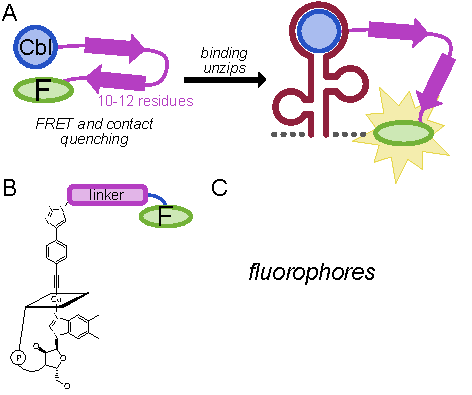
\includegraphics[width=\textwidth]{figures/aim1v2.pdf}

\end{centering}
\footnotesize
\caption{\label{figure:aim1}
A) Linkers. B) Conjugation sites. C) Fluorophores.
}
\end{wrapfigure}
%%%%%%%%%%%%%%%%%%%%%%%%%%%%%%%%%%%%%%%%%%%%%%%%%%%%%%%%%%%%%%%%%%%%%%%%%%%%%%%%

Ideally, in the unbound state, the cobalamin and fluorophore would be closely associated to maximize FRET and contact quenching.\cite{LeeDesignSynthesisCharacterization2009} In the RNA-bound state, the molecules would reside at their maximal distance to promote fluorescence. To strike this balance, I propose the use of a synthetic beta turn as the linker between cobalamin and the fluorophore (Fig. \ref{figure:aim1}A). Such a linker would hold the molecules close in solution, but would be linearized upon binding to the aptamer. A number of such beta turns have been developed. These motifs are as small as twelve amino acids and many are stable to denaturation up to 85 C.\cite{KierProbingLowerSize2008} In the unbound state, such a linker would hold the quencher and fluorophore in close proximity (due to the short distance between the N and C termini of the peptide). When the cobalamin is bound by an aptamer, steric occlusion would force the beta turn to unfold to place the fluorophore-quencher pair at a larger distance. The amino acids of the peptide linker will be varied to adjust the stability of the fold. \comment{More or less specific here? Discuss other linker possibilities?} The new constructs will be tested for their ability to quench fluorescence, and their fluorescence signal induction in the presence of the Riboglow aptamer.

Another underexplored variable of the original Riboglow probes is the linker attachment point. Though the 5' hydroxyl of the cobalamin ribose is the most accessible nucleophile on the structure, there exist several other possible sites of conjugation. Perhaps the second most common site is the axial ligand of the cobalt metal itself. Though many studies have taken advantage of the labile nature of certain alkyl modifications at this position,\cite{ShellVitaminB12Tunable2015} others have found alkynyl modifications to be stable to air and light.\cite{ChrominskiReductionfreesynthesisstable2013,RuetzMarkusPhenylethynylcobalaminLightStable2013} Following this precedent, I will synthesize a cobalamin with an alkyne handle attached to the cobalt metal center (Fig. \ref{figure:aim1}B). Such a molecule has already been synthesized in the lab of Dorota Gryko (see Gryko letter of support), and shown to be amenable to functionalization via dipolar azide-alkyne cycloaddition (AAC).\cite{ChrominskiVitaminB12Derivatives2014} The alkyne handle will be readily conjugated to a variety of linkers with terminal azides. \comment{More detail here?} These constructs will be evaluated for brightness in the presence and absence of the cobalamin aptamer.

%Fluorescence turn-on will also be modulated through changes to the cobalamin metal center. Changes to the electronic environment of the metal center will shift the absorption spectrum, enabling greater spectral overlap with the fluorophore to be quenched.\comment{[Cite]} As the \textit{de novo} synthesis of a molecule such as vitamin B12 would be a massive undertaking,\comment{[Cite]} I will target modifications that can be made through derivatization of the native structure. Without modification of the native ligand, variation of the axial position of cobalamin, and of the metal center itself should be straightforward. There is a large body of work that targets such modifications for the synthesis of so called ``antivitamins".\cite{KrautlerBernhardAntivitaminsB12Structure2015,ChrominskiReductionfreesynthesisstable2013} Through this undertaking, I will be in contact with Professor Dorota Gryko (see Gryko letter of support) one of the experts in this field.

The final variable in the molecular structure of the Riboglow probe is the fluorophore itself. The ideal probe would minimize cellular autofluorescence through the use of a red fluorophore with a high extinction coefficient. I believe that the Janelia Fluor series of dyes is perfectly suited for our application (see Lavis support letter).\cite{Grimmgeneralmethodfinetune2017a} \comment{Not sure how much else is needed here.}
%Previous work showed that probes were quenched by the cobalamin center to varying degrees. Quenching correlated somewhat with the spectral overlap of the fluorophore and cobalamin absorption.
% TODO is this 100% true? compare Cy5 excitation/emission with ATTO probes.
% TODO make a point here about how redder is better

\comment{Summary and alternate approaches here.}

\textbf{\underline{Aim 2.} Adapt Riboglow for superresolution imaging.}\\
Visualization of the lifecycle of single RNA transcripts as they move throughout the cell remains a holy grail of RNA imaging.\comment{[Cite]} Such a goal is possible via superresolution imaging and a probe with adequate photostability, and should be achievable with the Riboglow platform. With the wide variety of new probe constructs developed in Aim 1, changes will be made to the sequence of the cobalamin aptamer to increase fluorescence turn-on. A directed evolution screen for fluorescence brightness will identify optimal aptamer sequences that promote fluorescence signal induction.

%%%%%%%%%%%%%%%%%%%%%%%%%%%%%%%%%%%%%%%%%%%%%%%%%%%%%%%%%%%%%%%%%%%%%%%%%%%%%%%%
%Aim 2
\begin{wrapfigure}[25]{r}{10cm}
%\vspace{-0.2in}
\begin{centering}
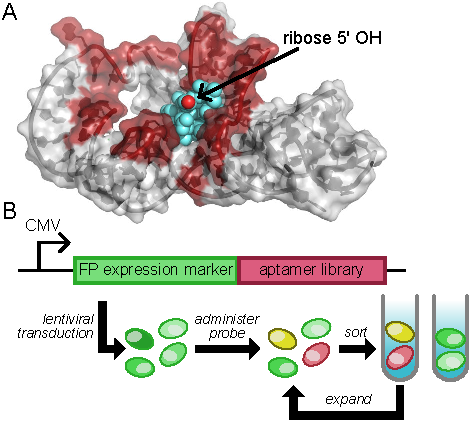
\includegraphics[width=\textwidth]{figures/aim2.pdf}

\end{centering}
\footnotesize
\caption{\label{figure:aim2}
A) Riboswitch sites for mutation will be targeted based on potential contact with the linker and fluorophore. PDB: 4FRN\cite{JohnsonJrB12cofactorsdirectly2012} B) RNA sequences will be screened for brightness relative to a fluorescent protein control.
}
\end{wrapfigure}
%%%%%%%%%%%%%%%%%%%%%%%%%%%%%%%%%%%%%%%%%%%%%%%%%%%%%%%%%%%%%%%%%%%%%%%%%%%%%%%%

First, a library will be designed that varies the environment surrounding the binding pocket of the cobalamin aptamer (Fig. \ref{figure:aim2}A). Though the guidance of Robert Batey (see Batey support letter), sites will be chosen to retain binding of the cobalamin, yet maximize the distance between the quencher and the fluorophore upon binding.\cite{JohnsonJrB12cofactorsdirectly2012} The Palmer lab is a leader in technologies for tool development in mammalian cells.\cite{FiedlerDropletMicrofluidicFlow2017,DeanHighSpeedMultiparameterPhotophysical2015} This expertise will be leveraged for screening libraries of cobalamin aptamers (Fig. \ref{figure:aim2}B). Libraries of transcripts will be transduced into mammalian cells, the probe of interest will be administered, and cells will be sorted via flow cytometry. Cells that show elevated brightness relative to a fluorescent protein expression control will be sequestered.
% QUESTION what is the absorption of Cbl bound to the riboswitch? does the spectrum change? Could we select for that?
In this way, libraries of up to one million members will be screened. Bright variants will be collected, cultured, and resubjected to sorting until only bright variants remain. Sequences will be evaluated through deep sequencing.

Candidate probes found through cell sorting will be verified in single molecule imaging experiments...

\comment{Summary and alternate approaches here.}

%%%%%%%%%%%%%%%%%%%%%%%%%%%%%%%%%%%%%%%%%%%%%%%%%%%%%%%%%%%%%%%%%%%%%%%%%%%%%%%%
%Aim 3: Multicomponent imaging
\begin{wrapfigure}[25]{l}{10cm}
%\vspace{-0.2in}
\begin{centering}
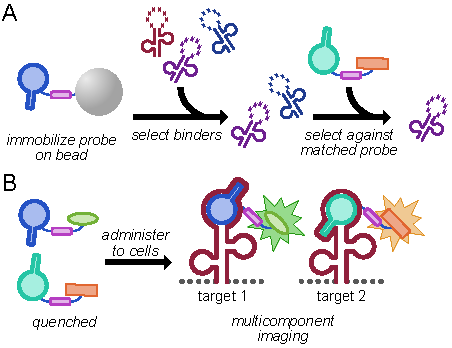
\includegraphics[width=\textwidth]{figures/aim3.pdf}
\end{centering}
\footnotesize
\caption{\label{figure:aim3}
A) SELEX will be used to screen for aptamers that bind each cobalamin in a mutually-exclusive manner. B) Mutually orthogonal cobalamin analogs will enable multicomponent RNA imaging. Signal turn-on will only be observed in the presence of the matched pair.
}
\end{wrapfigure}
%%%%%%%%%%%%%%%%%%%%%%%%%%%%%%%%%%%%%%%%%%%%%%%%%%%%%%%%%%%%%%%%%%%%%%%%%%%%%%%%

\textbf{\underline{Aim 3.} Develop mutually orthogonal Riboglow probes for multicomponent imaging.}\\
\comment{Don't forget Szostak precedent!\cite{LorschvitroselectionRNA1994}}
% TODO make a point here about how unnatural ligand architectures will help reduce off-target fluorescence.

%%% Local Variables: ***
%%% mode: latex ***
%%% TeX-master: "Research_and_SA.tex" ***
%%% End: ***


%%%%%%%%%%%%%%%%%%%%%%%%%%%%%%%%%%%%%%%%%%%%%%%%%%%%%%%%%%%%%%%%%%%%%%%%%%%%%%%%%%%%%%%%%%%%%%%%%%%%%%
% BIBLIOGRAPHY
%%%%%%%%%%%%%%%%%%%%%%%%%%%%%%%%%%%%%%%%%%%%%%%%%%%%%%%%%%%%%%%%%%%%%%%%%%%%%%%%%%%%%%%%%%%%%%%%%%%%%%

%%\eject

%\footnotesize
%\scriptsize
%\bibliographystyle{acm}
%%\bibliographystylesampl{nci}
\bibliographystyle{nci}
%\bibliographystyle{achemso}
%\bibliographystyle{nar}
%\bibliography{full}{sampl-r01}{BIBLIOGRAPHY AND REFERENCES CITED}
%\bibliography{sampl}{sampl-r01}{REFERENCES FROM PRIOR SAMPL CHALLENGES}

%%\bibliographysampl{sampl}
%%\eject
\bibliography{library}

\end{document}
